


\begin{frame}{\citetitle{MarcoNuno_Revista_2018_07_00} \footnotemark (1)}
%\begin{block}{Sistema de Posicionamiento Interior \footnotemark (1)} 
\begin{columns}
\begin{column}{0.5\textwidth}
		\begin{itemize}
		\item Determinar la ubicación de personas/objetos móviles en interiores es un problema abierto
		\item Se propuso un sistema basado en ML, para procesar las intensidades de señal de los puntos de acceso y de esta forma poder conocer la ubicación de manera precisa
		\end{itemize}
\end{column}
\begin{column}{0.3\textwidth}  
    \begin{center}
     %%%%% this is a minipage, so \textwidth is already adjusted to the size of the column
     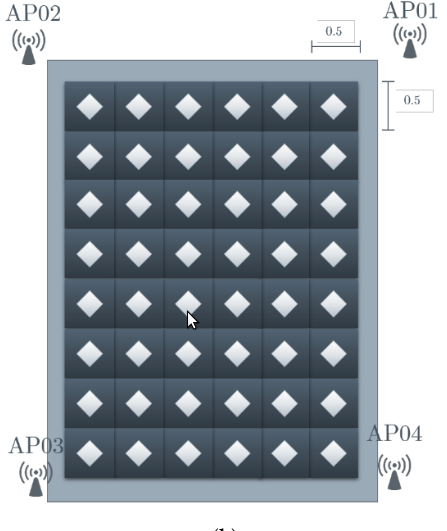
\includegraphics[width=0.85\textwidth]{Figs/IndoorPositionSystem2}
     \end{center}

\end{column}

\begin{column}{0.2\textwidth}  
    \begin{center}
     %%%%% this is a minipage, so \textwidth is already adjusted to the size of the column
     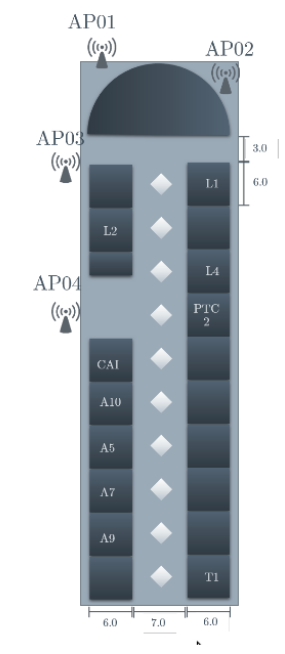
\includegraphics[width=0.8\textwidth]{Figs/IndoorPositionSystem1}
     \end{center}
\end{column}
\end{columns}
%\end{block} 
\footnotetext[1]{\fullcite{MarcoNuno_Revista_2018_07_00}}
\setcounter{footnote}{0}
\end{frame}

\begin{frame}{\citetitle{MarcoNuno_Revista_2018_07_00} \footnotemark (2)}
%\begin{block}{Sistema de Posicionamiento Interior (2)} 
\begin{columns}
\begin{column}{0.5\textwidth}
  \begin{center}
     %%%%% this is a minipage, so \textwidth is already adjusted to the size of the column
     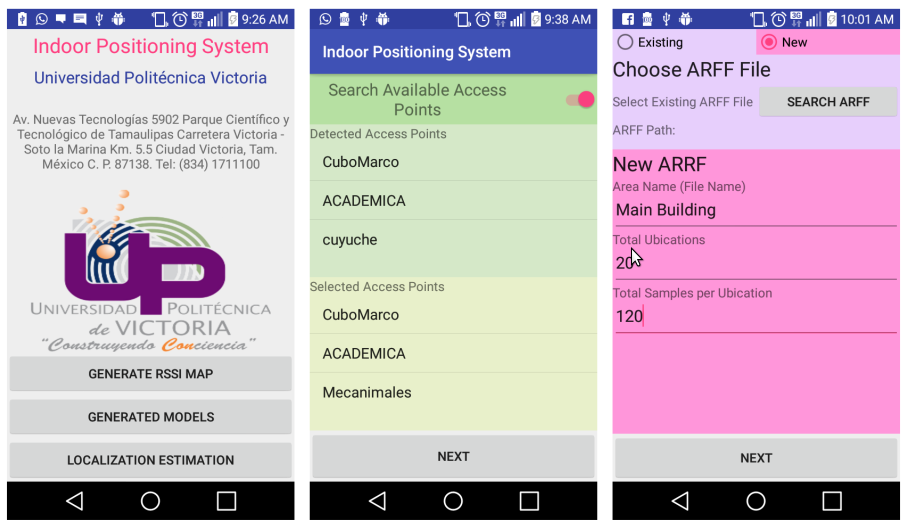
\includegraphics[width=0.95\textwidth]{Figs/IndoorPositionSystem3}
     %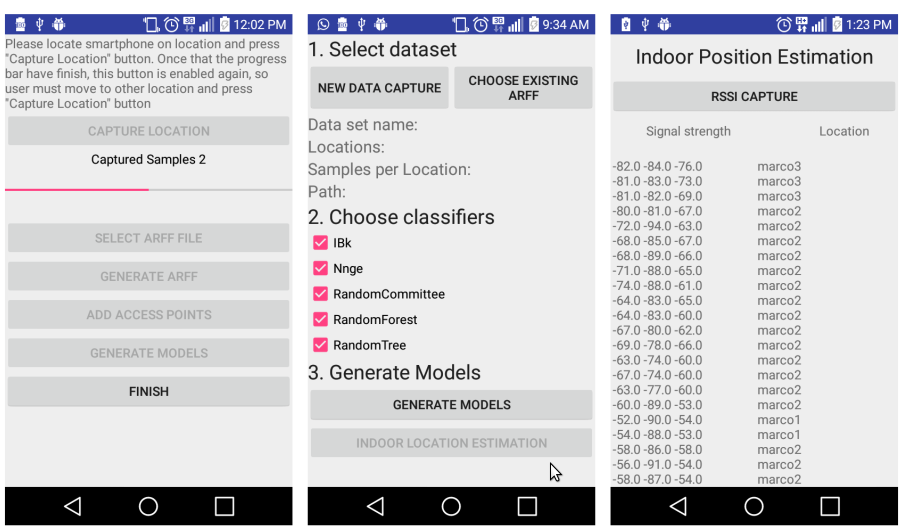
\includegraphics[width=0.5\textwidth]{Figs/IndoorPositionSystem4}
     \end{center}

\end{column}
\begin{column}{0.5\textwidth}
  \begin{center}
     %%%%% this is a minipage, so \textwidth is already adjusted to the size of the column
     %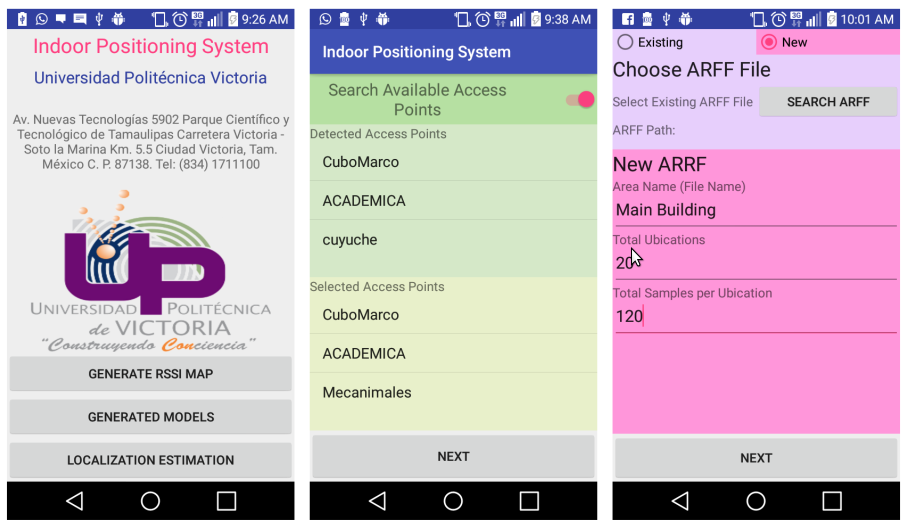
\includegraphics[width=0.5\textwidth]{Figs/IndoorPositionSystem3}
     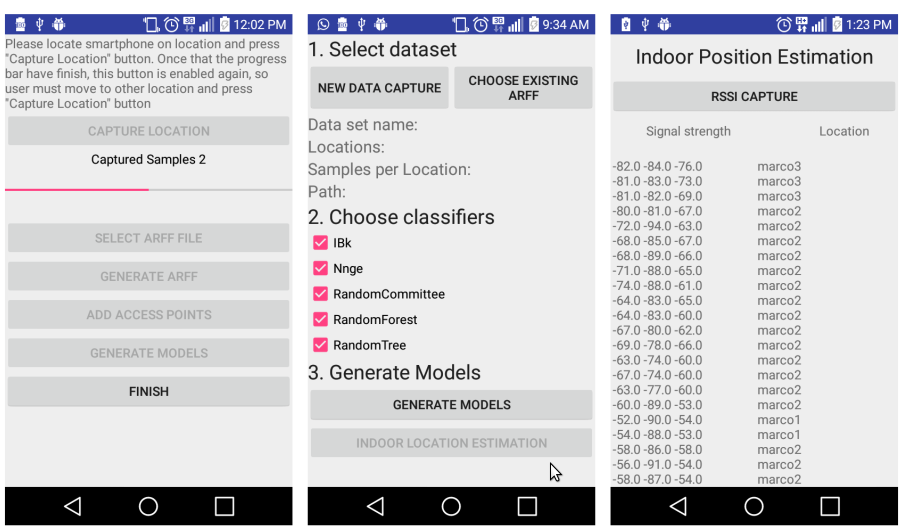
\includegraphics[width=0.95\textwidth]{Figs/IndoorPositionSystem4}
     \end{center}

\end{column}

\end{columns}



%\end{block} 
\end{frame}




